\subsection{Linux kernel source code}

\begin{frame}
  \frametitle{Programming language}
  \begin{itemize}
  \item Implemented in C like all UNIX systems
  \item A little Assembly is used too:
    \begin{itemize}
    \item CPU and machine initialization, exceptions
    \item Critical library routines.
    \end{itemize}
  \item No C++ used, see \url{http://vger.kernel.org/lkml/\#s15-3}
  \item All the code compiled with gcc
    \begin{itemize}
    \item Many gcc specific extensions used in the kernel code, any
      ANSI C compiler will not compile the kernel
    \item See
      \url{https://gcc.gnu.org/onlinedocs/gcc-10.2.0/gcc/C-Extensions.html}
    \end{itemize}
    \item Ongoing work to compile the kernel with the LLVM C compiler
      (Clang) too: \url{https://clangbuiltlinux.github.io/}
    \item There are also plans to create new code in Rust too:
      \url{https://lwn.net/Articles/829858/}
  \end{itemize}
\end{frame}

\begin{frame}
  \frametitle{No C library}
  \begin{itemize}
  \item The kernel has to be standalone and can't use user space code.
  \item Architectural reason: user space is implemented on top of kernel services, not the
    opposite.
  \item Technical reason: the kernel is on its own during the boot up
    phase, before it has accessed a root filesystem.
  \item Hence, kernel code has to supply its own library implementations
    (string utilities, cryptography, uncompression...)
  \item So, you can't use standard C library functions in kernel code
    (\code{printf()}, \code{memset()}, \code{malloc()},...).
  \item Fortunately, the kernel provides similar C functions for your
    convenience, like \kfunc{printk}, \kfunc{memset},
    \kfunc{kmalloc}, ...
  \end{itemize}
\end{frame}

\begin{frame}
  \frametitle{Portability}
  \begin{itemize}
  \item The Linux kernel code is designed to be portable
  \item All code outside \kdir{arch} should be portable
  \item To this aim, the kernel provides macros and functions to
    abstract the architecture specific details
    \begin{itemize}
    \item Endianness
    \item I/O memory access
    \item Memory barriers to provide ordering guarantees if needed
    \item DMA API to flush and invalidate caches if needed
    \end{itemize}
  \item Never use floating point numbers in kernel code. Your code may
    need to run on a low-end processor without a floating point unit.
  \end{itemize}
\end{frame}

\begin{frame}
  \frametitle{Linux internal API/ABI instability}
  \begin{columns}
    \column{0.7\textwidth}
    Linux internal API is not stable
    \begin{itemize}
    \item The source code of a driver is not portable across versions
      \begin{itemize}
      \item In-tree drivers are updated by the developer proposing the API
        change: works great for mainline code
      \item An out-of-tree driver compiled for a given version may no
        longer compile or work on a more recent one
      \item See \kdochtml{process/stable-api-nonsense} for reasons why
      \end{itemize}
    \end{itemize}
    Linux internal ABI is not stable
    \begin{itemize}
    \item A binary module compiled for a given kernel version cannot be
      used with another version
      \begin{itemize}
      \item The module loading utilities will perform this check prior
        to the insertion
      \end{itemize}
    \end{itemize}
    \column{0.3\textwidth}
    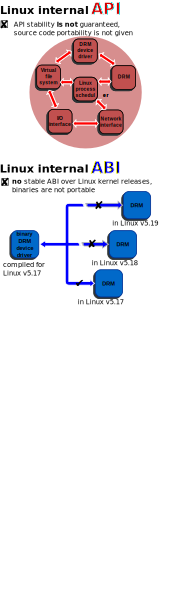
\includegraphics[height=0.8\textheight]{slides/kernel-source-code-drivers/linux-internal-api.pdf}
    \tiny
    Modified Image from Wikipedia:\\
    \url{https://bit.ly/2U2rdGB}
  \end{columns}
\end{frame}

\begin{frame}
  \frametitle{Linux kernel to user API/ABI stability}
  \begin{columns}
    \column{0.7\textwidth}
    Linux kernel to userspace API is stable
    \begin{itemize}
    \item Source code for userspace applications will not have to be
      updated when compiling for a more recent kernel
      \begin{itemize}
      \item System calls, \code{/proc} and \code{/sys} content cannot be
        removed or changed. Only new entries can be added.
      \end{itemize}
    \end{itemize}
    Linux kernel to userspace ABI is stable
    \begin{itemize}
    \item Binaries are portable and can be executed on a more recent
      kernel
      \begin{itemize}
      \item The way memory is accessed, the size of the variables in
        memory, how structures are organized, the calling convention,
        etc, are all stable over time.
      \end{itemize}
    \end{itemize}
    \column{0.3\textwidth}
    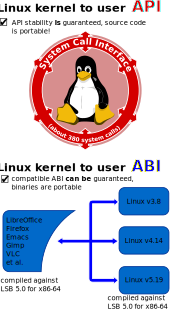
\includegraphics[height=0.8\textheight]{slides/kernel-source-code-drivers/linux-user-api.pdf}
    \tiny
    Modified Image from Wikipedia:\\
    \url{https://bit.ly/2U2rdGB}
  \end{columns}
\end{frame}

\begin{frame}
  \frametitle{Kernel memory constraints}
  \begin{itemize}
  \item No memory protection
  \item The kernel doesn't try to recover from attemps to access illegal
    memory locations. It just dumps {\em oops} messages on the system console.
  \item Fixed size stack (8 or 4 KB). Unlike in user space, no mechanism
    was implemented to make it grow. Don't use recursion!
  \item Swapping is not implemented for kernel memory either\\
    (except {\em tmpfs} which lives completely in the page cache and on swap)
  \end{itemize}
\end{frame}

\begin{frame}
  \frametitle{Linux kernel licensing constraints}
  \begin{itemize}
  \item The Linux kernel is licensed under the GNU General Public
    License version 2
    \begin{itemize}
    \item This license gives you the right to use, study, modify and
      share the software freely
    \end{itemize}
  \item However, when the software is redistributed, either modified
    or unmodified, the GPL requires that you redistribute the software
    under the same license, with the source code
    \begin{itemize}
    \item If modifications are made to the Linux kernel (for example
      to adapt it to your hardware), it is a derivative work of the
      kernel, and therefore must be released under GPLv2.
    \end{itemize}
  \item The GPL license has been successfully enforced in courts:
    \url{https://en.wikipedia.org/wiki/Gpl-violations.org\#Notable\_victories}
  \item However, you're only required to do so
    \begin{itemize}
    \item At the time the device starts to be distributed
    \item To your customers, not to the entire world
    \end{itemize}
  \end{itemize}
\end{frame}

\begin{frame}
  \frametitle{Proprietary code and the kernel}
  \begin{columns}
    \column{0.75\textwidth}
  \begin{itemize}
  \item It is illegal to distribute a binary kernel that includes
    statically compiled proprietary drivers
  \item The kernel modules are a gray area: are they derived works of
    the kernel or not?
    \begin{itemize}
    \item The general opinion of the kernel community is that
      proprietary modules are bad: \kdochtml{process/kernel-driver-statement}
    \item From a legal point of view, each driver is probably a
      different case
    \item Is it really useful to keep your drivers secret?
    \end{itemize}
  \item There are some examples of proprietary drivers, like the
    Nvidia graphics drivers
    \begin{itemize}
    \item They use a wrapper between the driver and the kernel
    \item Unclear whether it makes it legal or not
    \item Pre-compiled drivers work with only one kernel version, kernel
      updates, even minors, might just become impossible.
    \end{itemize}
  \end{itemize}
    \column{0.25\textwidth}
    \includegraphics[height=0.85\textheight]{slides/kernel-source-code-drivers/binary-blobs.pdf}
  \end{columns}
\end{frame}

\begin{frame}
  \frametitle{Advantages of GPL drivers}
  \begin{itemize}
  \item You don't have to write your driver from scratch. You can
    reuse code from similar free software drivers.
  \item Your drivers can be freely and easily shipped by others (for
    example by Linux distributions or embedded Linux build systems).
  \item Legal certainty, you are sure that a GPL driver is fine from a
    legal point of view.
  \end{itemize}
\end{frame}

\begin{frame}
  \frametitle{Advantages of mainlining your kernel drivers}
  \begin{itemize}
  \item The community, reviewers and maintainers will review your code
    before accepting it, offering you the opportunity to enhance it and
    understand better the internal APIs.
  \item Once accepted, you will get cost-free bug and security fixes,
    support for new features, and general improvements.
  \item Your work will automatically follow the API changes.
  \item Accessing your code will be much easier for users.
  \item Your code will remain valid no matter the kernel version.
  \end{itemize}
  This will for sure reduce your maintenance and support work
\end{frame}

\begin{frame}
  \frametitle{User space device drivers 1/3}
  \begin{itemize}
  \item In some cases, it is possible to implement device drivers in
    user space!
  \item Can be used when
    \begin{itemize}
    \item The kernel provides a mechanism that allows user space
      applications to directly access the hardware.
    \item There is no need to leverage an existing kernel subsystem
      such as the networking stack or filesystems.
    \item There is no need for the kernel to act as a ``multiplexer''
      for the device: only one application accesses the device.
    \end{itemize}
  \end{itemize}
\end{frame}

\begin{frame}
  \frametitle{User space device drivers 2/3}
  \begin{itemize}
  \item Possibilities for user space device drivers:
    \begin{itemize}
    \item USB with {\em libusb}, \url{https://libusb.info/}
    \item SPI with {\em spidev}, \kdochtml{spi/spidev}
    \item I2C with {\em i2cdev}, \kdochtml{i2c/dev-interface}
    \item Memory-mapped devices with {\em UIO}, including interrupt
      handling, \kdochtml{driver-api/uio-howto}
    \end{itemize}
  \item Certain classes of devices (printers, scanners, 2D/3D graphics
    acceleration) are typically handled partly in kernel space, partly
    in user space.
  \end{itemize}
\end{frame}

\begin{frame}
  \frametitle{User space device drivers 3/3}
  \begin{itemize}
  \item Advantages
    \begin{itemize}
    \item No need for kernel coding skills.
    \item Drivers can be written in any language, even Perl!
    \item Drivers can be kept proprietary.
    \item Driver code can be killed and debugged. Cannot crash the
      kernel.
    \item Can use floating-point computation.
    \item Potentially higher performance, especially for
      memory-mapped devices, thanks to the avoidance of system calls.
    \end{itemize}
  \item Drawbacks
    \begin{itemize}
    \item Missing hardware abstraction provided by the kernel, need
          to adapt applications when replacing one device by another.
    \item Less straightforward to handle interrupts.
    \item Increased interrupt latency.
    \end{itemize}
  \end{itemize}
\end{frame}
